\section{Validation}

\subsection{Co-Simulation Setup}
The simulation validation was conducted on the TruckSim--STAR-CCM+ vehicle--liquid coupling platform reported in \cite{KomasaQi2025AntiRollover_TITS}. The vehicle is the default full-load 49-ton 3A sleeper tractor with trailer. The tank is filled to 50\%, and the liquid--vehicle interaction is generated by a three-dimensional STAR-CCM+ sloshing model coupled with the nonlinear TruckSim vehicle model. This high-fidelity platform is used only for validation; the proposed Q-band controller does not use the liquid states, trailer-side states, or real-time fluid forces as feedback.

The main comparison uses one continuous five-pins maneuver. The longitudinal speed increases linearly from 60 km/h to 100 km/h within 60 s, covering the lower and upper highway speed limits for trucks. The five double-lane-change (DLC) maneuvers become progressively more aggressive: the two lane changes within DLC1--DLC5 are completed over longitudinal distances of 100, 81.25, 62.5, 43.75, and 25 m, respectively. Therefore, the last pins simultaneously impose higher speed, shorter lane-change distance, and stronger lateral excitation.

Three controllers are compared. The first is the built-in TruckSim preview tracking (PT), which tracks the reference path without considering rollover risk. The second is the full-state active rollover tracking controller (Full-ART) from \cite{KomasaQi2025AntiRollover_TITS}, which explicitly uses the trailer and liquid dynamics and requires liquid-state observation together with trailer-state feedback. This method can drive the vehicle closer to its physical handling limit, but its online model, calibration, and sensing requirements are high. The third is the proposed Q-band ART, which uses only tractor-side motion information and suppresses dangerous lateral-excitation frequency bands. The comparison is intended to show whether a low-observability controller can approach the anti-rollover performance of the full-state method.

\begin{figure*}[!htbp]
\centering
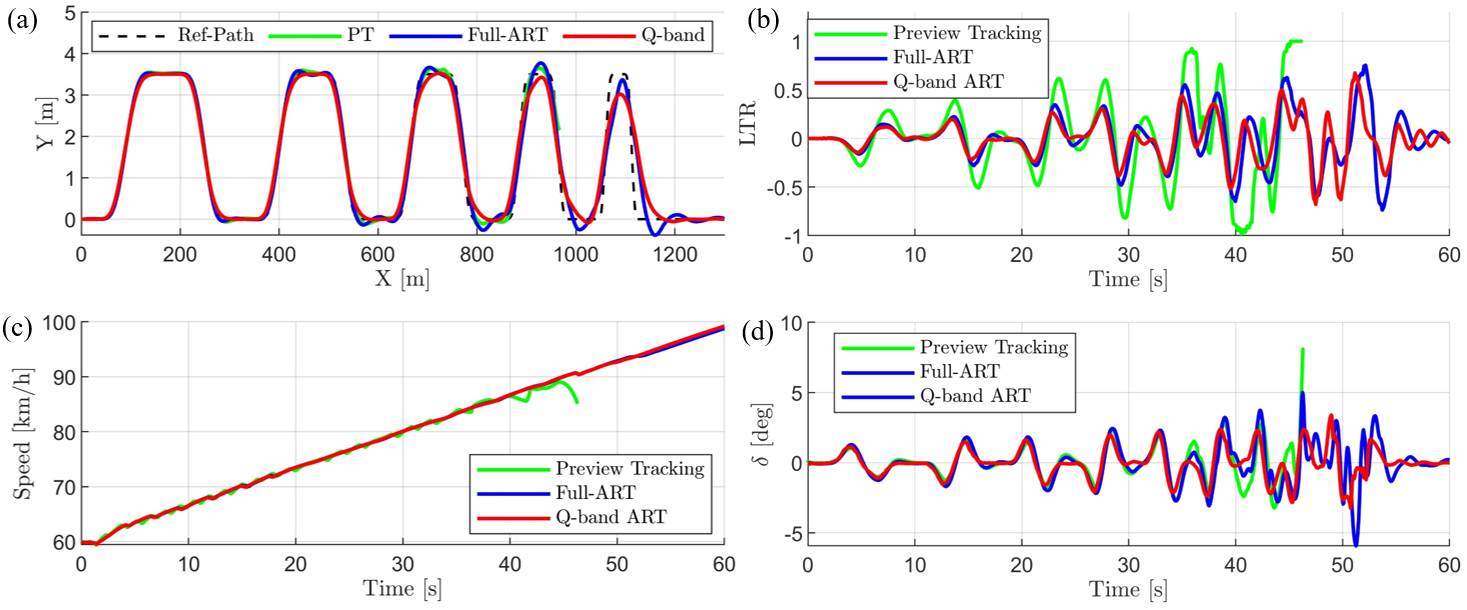
\includegraphics[width=1.0\textwidth]{fig/pin5_sim_results.png}
\caption{Continuous five-pins comparison: (a) trajectory tracking, (b) lateral load transfer ratio, (c) longitudinal speed, and (d) front steering angle. PT denotes the TruckSim preview tracking baseline, Full-ART denotes the full-state active rollover tracking controller in \cite{KomasaQi2025AntiRollover_TITS}, and Q-band ART denotes the proposed controller.}
\label{fig:pin5_sim_results}
\end{figure*}

\begin{figure*}[!htbp]
\centering
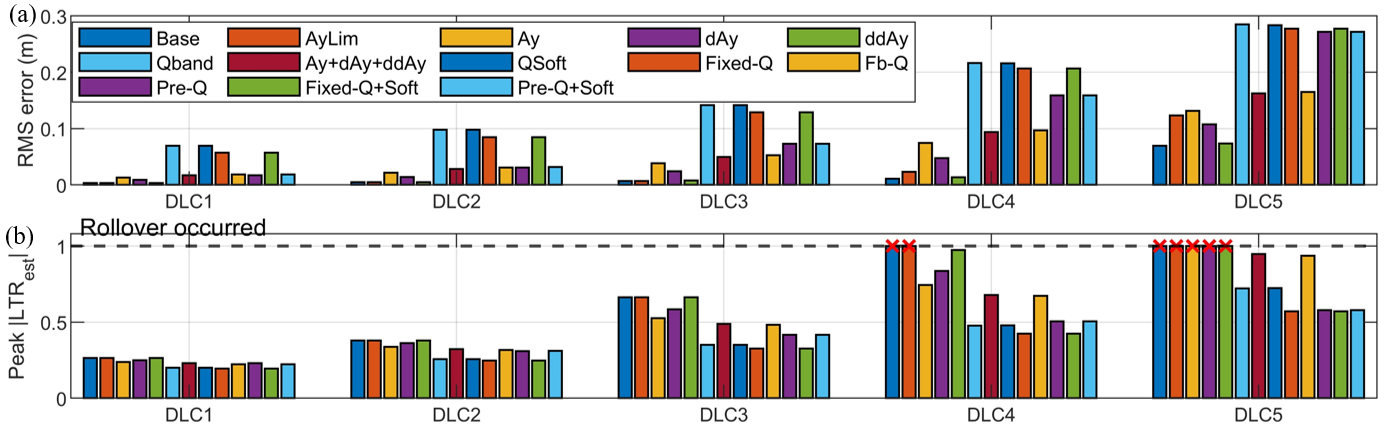
\includegraphics[width=0.98\textwidth]{fig/ablation.png}
\caption{Ablation study of the Q-band mechanism in five independent DLC segments: (a) RMS tracking error and (b) peak estimated LTR. Red crosses at the dashed $|\LTR_{\mathrm{est}}|=1$ line indicate simulations in which rollover occurred, not numerical clipping.}
\label{fig:ablation}
\end{figure*}

\subsection{Continuous Five-Pins Results}
Figure~\ref{fig:pin5_sim_results} shows the continuous five-pins comparison. PT follows the first several pins tightly, but it keeps pursuing the geometric path after the maneuver becomes dynamically unsafe. Its LTR increases rapidly in the later pins and reaches the rollover boundary at approximately 46 s, after which the simulation cannot continue as a physically valid run. This confirms that pure preview tracking is inadequate for a high-speed liquid tank semi-trailer, even when the reference path itself is smooth.

Full-ART and Q-band ART both complete the 60 s maneuver without rollover. Full-ART achieves slightly tighter path tracking in the most aggressive pins because it uses a richer vehicle--liquid prediction model and full-state feedback. In contrast, Q-band ART intentionally relaxes the path in high-risk portions, especially near the fifth pin, so that the lateral excitation does not continue feeding the dominant roll--sloshing bands. The resulting trajectory is slightly more conservative, but the LTR response remains comparable to that of Full-ART for most of the maneuver. The speed curves of Full-ART and Q-band ART nearly overlap, indicating that the comparison is not biased by different speed histories. The steering-angle response also remains within practical bounds; Q-band ART reduces the most dangerous oscillatory steering content rather than relying on abrupt large steering reversals.

These results highlight the main tradeoff of the proposed method. Full-ART can exploit a detailed trailer--liquid model to approach the vehicle limit more aggressively, but this requires information that is difficult to obtain on production vehicles. Q-band ART sacrifices a small amount of geometric tracking tightness and instead obtains a similar rollover-prevention effect using only simple tractor-side measurements and a low-order prediction model.

\subsection{Q-Band Ablation Study}
The ablation study is conducted with five independent DLC simulations rather than one continuous trajectory. This choice is necessary because, once a controller rolls the vehicle over in an earlier pin, the subsequent pins are no longer physically meaningful. For each DLC, the initial speed and pose are reset to the corresponding rollover-free Q-band condition at the entrance of the segment. The compared variants include tracking only (Base), lateral-acceleration amplitude limitation (AyLim), acceleration magnitude and difference penalties, fixed Q-band weighting, feedback-adjusted Q-band weighting, preview Q-band weighting, and soft-constrained Q-band combinations.


Figure~\ref{fig:ablation} summarizes the ablation results. In DLC1 and DLC2, all variants are far from the rollover boundary, and the tracking errors remain small. This indicates that the additional Q-band terms do not unnecessarily dominate the controller in low-risk maneuvers. As the lane-change distance decreases in DLC3, the difference between amplitude-based regulation and frequency-selective regulation becomes visible. The variants that include Q-band weighting reduce the peak $|\LTR_{\mathrm{est}}|$ while keeping the RMS tracking error within an acceptable range.

The difference becomes decisive in DLC4 and DLC5. The Base controller and several acceleration-only variants reach the rollover boundary. Importantly, AyLim uses the same lateral-acceleration amplitude limitation, yet it still rolls over in the severe segments. Therefore, rollover prevention cannot be explained by limiting only the peak value of $a_y$. Even when the acceleration magnitude is bounded, repeated excitation near the dominant roll--sloshing bands can accumulate energy and trigger rollover. This observation directly supports the Q-band theory: the dangerous part is not only the acceleration amplitude, but also its frequency content over the preview horizon.

Among the Q-band variants, fixed Q-band weighting already reduces the peak LTR in the severe DLCs, showing that the frequency-selective penalty is the core contributor. The soft-constrained variants further improve robustness by allowing controlled tracking relaxation when the maneuver approaches the roll limit. Preview-adaptive weighting is particularly useful in DLC4 and DLC5 because it increases the dangerous-band penalty before the vehicle enters the strongest lane-change excitation. Feedback adjustment and residual memory provide an additional safety margin when the measured response shows amplified output in a band that is being excited by the steering input. Overall, the ablation confirms that the main protective mechanism is the suppression of lateral excitation energy in the dangerous frequency bands, while preview scheduling and soft constraints determine how early and how smoothly this protection is activated.

% TODO（作者）：最终稿若需要更强定量性，可从 MATLAB 结果表补入 DLC4/DLC5 中 Q-band ART 相对 Base、AyLim 和 Full-ART 的峰值 LTR 降低百分比，以及 RMS 误差增加量。

\subsection{Model-Truck Experiment}
The 1:14 semi-trailer tank truck experiment was conducted to verify that the Q-band mechanism remains effective on a physical platform. The experiment used a double-lane-change or 5-pins-like reference path scaled according to the model-truck operating envelope. Baseline tracking and Q-band ART were compared under the same speed and filling-rate settings. The measured responses include path tracking, steering command, lateral acceleration, roll/yaw response, liquid-surface motion when available, and controller solve time.

The model-truck results show the same qualitative behavior as the simulation. Baseline tracking follows the reference more tightly but excites larger roll-slosh motion, and the anti-roll support/contact or rollover-risk proxy reaches xxx. Q-band ART reduces the peak risk proxy by xxx\%, keeps the liquid/roll response within xxx, and increases RMS tracking error from xxx m to xxx m. The controller average and peak solve times are xxx ms and xxx ms, respectively, satisfying the real-time requirement of the experimental platform.

% TODO（作者）：这里后续需要插入模型车实验总图。建议包含：平台照片、实验路径、baseline vs Q-band 轨迹、风险代理LTR、液面或侧倾响应、求解时间。若没有可靠液面识别，就明确写 liquid-surface motion is used only for qualitative video confirmation.
\begin{table}[!t]
\caption{Validation Summary With Replaceable Results}
\label{tab:validation_summary}
\centering
\begin{tabularx}{\linewidth}{lXXX}
\toprule
Case & Rollover result & Tracking result & Online information\\
\midrule
PT simulation & rollover at 46 s & tight before rollover & tractor states\\
Full-ART simulation & no rollover & tightest near limit & tractor, trailer, and liquid states\\
Q-band ART simulation & no rollover & slightly conservative & tractor states only\\
Model-truck baseline & xxx & xxx & --\\
Model-truck Q-band ART & xxx & xxx & xxx ms\\
\bottomrule
\end{tabularx}
\end{table}
% TODO（作者）：若最终表格需要定量指标，可将 rollover result 替换为 peak |LTR_est| 或模型车风险代理；仿真和模型车若指标定义不同，应在表注中说明。
